
\chapter[Dạng bài: Quá trình biến đổi lực\\ của con lắc đơn không chịu tác dụng\\ của ngoại lực khác trọng lực]{Dạng bài: Quá trình biến đổi lực của con lắc đơn không chịu tác dụng của ngoại lực khác trọng lực}
\section{Lý thuyết}
\subsection{Lực căng dây}
\begin{equation*}
	T = mg (3\cos \alpha - 2 \cos \alpha_0)
\end{equation*}
\begin{itemize}
	\item Khi vật đi qua vị trí cân bằng, lực căng dây là lớn nhất:
	\begin{equation*}
		T_{\text{max}} =mg (3 -2 \cos \alpha_0)
	\end{equation*}
	\item Khi vật qua vị trí biên, lực căng dây là nhỏ nhất:
	\begin{equation*}
		T_{\text{min}} =mg \cos \alpha_0
	\end{equation*}
\end{itemize}
\begin{center}
	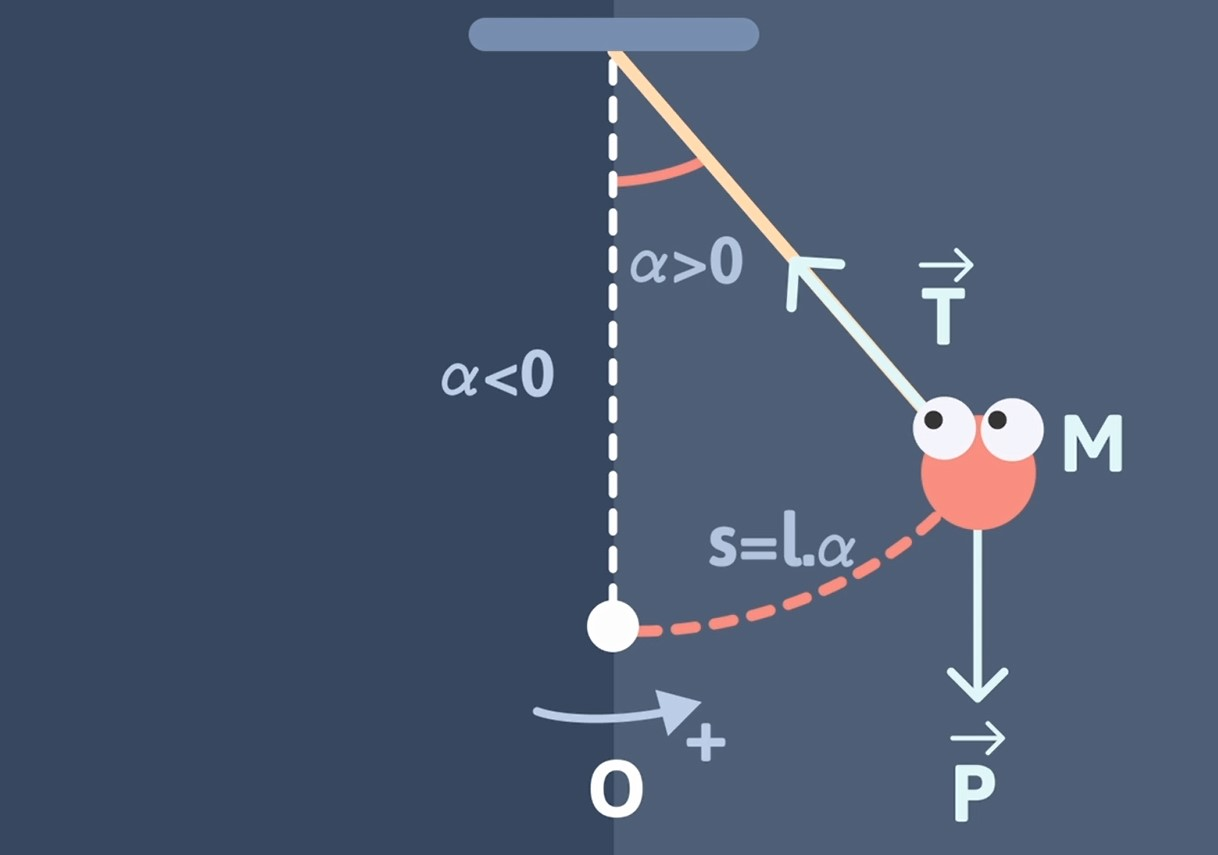
\includegraphics[scale=0.3]{../figs/VN12-PH-04-A-003-2-V2-1.jpg}
\end{center}
\subsection{Con lắc trùng phùng}
Hiện tượng con lắc trùng phùng là hai con lắc có cùng li độ và chuyển động cùng chiều sau một khoảng thời gian nhất định.

Gọi $T_1$ chu kỳ dao động nhỏ của con lắc thứ nhất, $T_2$ là chu kỳ dao động nhỏ của con lắc thứ hai, $\theta$ là khoảng thời gian giữa hai lần trùng phùng liên tiếp. Ta có:
\begin{itemize}
	\item Nếu $T_1 >T_2$: \begin{equation*}\dfrac{1}{T_2} = \dfrac{1}{T_1} +\dfrac{1}{\theta}.\end{equation*}
	\item Nếu $T_1 <T_2$: \begin{equation*}\dfrac{1}{T_2} = \dfrac{1}{T_1} -\dfrac{1}{\theta}.\end{equation*}
	\item Khoảng thời gian giữa 2 lần trùng phùng liên tiếp:
	\begin{equation*}
		\theta =\dfrac{T_1T_2}{|T_1-T_2|}.
	\end{equation*}
\end{itemize}
\subsection{Con lắc đứt dây khi qua vị trí cân bằng}
Khi qua vị trí cân bằng, vận tốc con lắc có phương nằm ngang, nên nếu dây đứt thì vật nặng sẽ chuyển động ném ngang. 
\begin{center}
	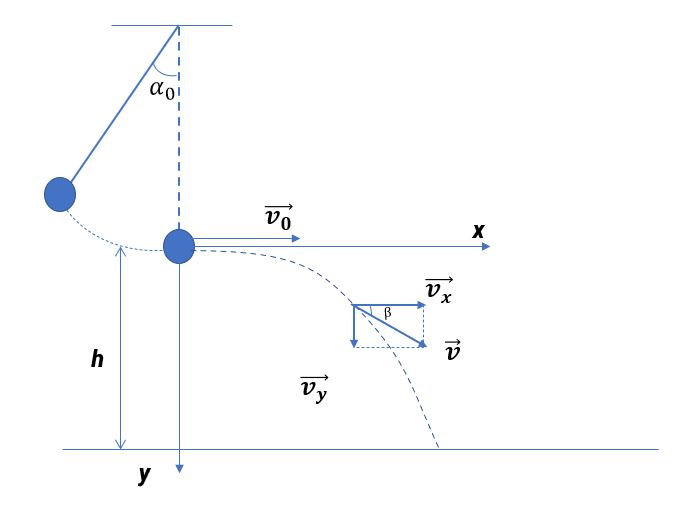
\includegraphics[scale=0.6]{../figs/VN12-PH-04-A-003-2-V2-2.JPG}
\end{center}
\begin{itemize}
	\item Tốc độ quả cầu khi dây đứt:
	\begin{equation*}
		v_0 = \sqrt{2gl(1-\cos \alpha_0)}.
	\end{equation*}
	\item Phương trình chuyển động của chuyển động ném ngang (với gốc tọa độ tại vị trí cân bằng như hình vẽ):
	\begin{equation*}
		\begin{cases}
			x=v_0t.\\
			y=\text{0,5} gt^2
		\end{cases}.
	\end{equation*}
	\item Khi chạm đất:
	\begin{equation*}
		\begin{cases}
			x_{\text{c}}=v_0t_{\text{c}}.\\
			y=h\Rightarrow \text{0,5} gt^2=h \Rightarrow t_{\text{c}} =\sqrt {\dfrac{2h}{g}}
		\end{cases}.
	\end{equation*}
	\item Các thành phần vận tốc:
	\begin{equation*}
		\begin{cases}
			v_{\text{x}} =x' =(v_0t)'=v_0 \\
			v_{\text{y}} =y' = (\text{0,5} gt^2)'=gt
		\end{cases}.
	\end{equation*}
	\begin{equation*}
		\Rightarrow
		\begin{cases}
			\tan \beta =\dfrac{v_{\text{y}}}{v_{\text{x}}}=\dfrac{gt}{v_0}\\
			v=\sqrt{v^2_{\text{x}}+v^2_{\text{y}}}
		\end{cases}.
	\end{equation*}
	\item Quỹ đạo của quả nặng sau khi đứt dây tại VTCB là một Parabol.
\end{itemize}
\section{Mục tiêu bài học - Ví dụ minh họa}
\begin{dang}{Vận dụng được công thức xác định\\ lực căng dây}
	\viduii{2}
	{
		Một con lắc đơn gồm vật có khối lượng $100\ \text g$, chiều dài dây $l=40\ \text{cm}$. Kéo vật ra khỏi VTCB để dây treo hợp với phương thẳng đứng một góc $30^\circ$ rồi buông tay. Lấy $g=10\ \text{m/s}^2$. Lực căng của dây treo khi vật qua vị trí cao nhất là
		\begin{mcq}(4)
			\item $0,2\ \text{N}$.
			\item $0,5\ \text{N}$.
			\item $\dfrac{\sqrt{3}}{2}\ \text{N}$.
			\item $\dfrac{\sqrt{3}}{5}\ \text{N}$.
		\end{mcq}
	}
	{\begin{center}
			\textbf{Hướng dẫn giải}
		\end{center}
		
		Vị trí cao nhất là vị trí biên, khi đó:
		$$T_{\text{min}} =mg \cos \alpha_0 = \dfrac{\sqrt{3}}{2}\ \text{N}$$
		
		\textbf{Đáp án: C.}
	}
	\viduii{3}
	{
		Một con lắc đơn dao động điều hòa với phương trình li độ dài $s=2 \cos 7t\ \text{cm}$, với $t$ tính bằng giây. Tại nơi có gia tốc trọng trường $g=9,8\ \text{m/s}^2$, tỉ số giữa lực căng dây và trọng lực tác dụng lên quả cầu ở vị trí cân bằng là
		\begin{mcq}(4)
			\item $1,08$.
			\item $0,95$.
			\item $1,01$.
			\item $1,05$.
		\end{mcq}
	}
	{
		\begin{center}
			\textbf{Hướng dẫn giải}
		\end{center}
		Ta có $\omega = \dfrac{g}{l}=7\ \text{rad}\Rightarrow l = 0,2\ \text m$
		Ở vị trí cân bằng thì lực căng dây là
		$$T_{\text{max}} =mg (3 -2 \cos \alpha_0)$$
		
		Tỉ số giữa $T_\text{max}$ và trọng lực $P$ là
		$$\dfrac{T_\text{max}}{P}=\dfrac{mg (3 -2 \cos \alpha_0)}{mg}=1,01$$
		
		\textbf{Đáp án: C.}
	}
\end{dang}
\begin{dang}{Xác định được chu kỳ trùng phùng\\ của con lắc đơn}
	\viduii{2}
	{
		Hai con lắc đơn treo cạnh nhau có chu kì dao động nhỏ là $T_1=4\ \text s$ và $T_2=4,8\ \text s$. Kéo hai con lắc lệch một góc nhỏ như nhau rồi đồng thời buông nhẹ. Hỏi sau thời gian ngắn nhất là bao nhiêu thì hai con lắc sẽ đồng thời trở lại vị trí này?
		\begin{mcq}(4)
			\item $8,8\ \text{s}$.
			\item $12\ \text{s}$.
			\item $6,248\ \text{s}$.
			\item $24\ \text{s}$.
		\end{mcq}
	}
	{\begin{center}
			\textbf{Hướng dẫn giải}
		\end{center}
		
		Áp dụng công thức chu kỳ của con lắc trùng phùng:
		$$\theta = \dfrac{T_1T_2}{|T_1 - T_2|} = 24\ \text s$$
		
		\textbf{Đáp án: D.}
	}
	\viduii{3}
	{
		Cho hai con lắc đơn A và B dao động điều hòa trên hai đường thẳng song song với nhau. Ban đầu kéo vật nặng của hai con lắc về cùng một phía hợp với phương thẳng đứng một góc bằng nhau rồi buông nhẹ cùng một lúc. Biết rằng chu kì dao động của con lắc B nhỏ hơn chu kì dao động của con lắc A. Người ta đo được sau 4 phút 30 giây thì thấy hai vật nặng lại trùng nhau ở vị trí ban đầu. Biết chu kì dao động của con lắc A là $0,5\ \text s$. Tỉ số chiều dài của con lắc A so với con lắc B là
		\begin{mcq}(4)
			\item $1,0037$.
			\item $1,0022$.
			\item $1,0026$.
			\item $0,9962$.
		\end{mcq}
	}
	{
		\begin{center}
			\textbf{Hướng dẫn giải}
		\end{center}
		
		Gọi $T_1$ là chu kì dao động của con lắc A, $T_2$ là chu kì dao động của con lắc B.
		
		Ta có khoảng thời gian trùng phùng: $$\theta = nT_1 = (n+1)T_2 \Rightarrow 270 = n\cdot 0,5 \Rightarrow n=540$$
		$$\Rightarrow T_2 = \dfrac{n}{n+1}T_1 = 0,499\ \text s$$
		
		Mà $T=2\pi \sqrt{\dfrac{l}{g}}\Rightarrow \dfrac{l_1}{l_2} = \left(\dfrac{T_1}{T_2}\right)^2 = 1,0037$
		
		\textbf{Đáp án: A.}
	}
\end{dang}
\begin{dang}{Liên hệ được bài toán con lắc đơn đứt dây với bài toán ném ngang}
	\viduii{3}{
		Một con lắc đơn gồm một quả cầu có $m = 20\ \text{g}$ được treo vào một dây dài $l = 1\ \text{m}$. Lấy $g=10\ \text{m/s}^2$. Bỏ qua ma sát. Kéo con lắc khỏi VTCB một góc $30^\circ$ rồi buông không vận tốc đầu. Khi qua VTCB một lần nào đó dây bị đứt. Hỏi quả cầu chạm đất cách VTCB bao xa (tính theo phương ngang)? Biết VTCB cách mặt đất 1,2 m.
	}{
		\begin{center}
			\textbf{Hướng dẫn giải}
		\end{center}
		Vận tốc ban đầu:
		\begin{equation*}
			v_0 = \sqrt{2gl(1-\cos \alpha_0)}= \text{1,64}\ \text{m/s}.
		\end{equation*}
		Thời gian chạm đất:
		\begin{equation*}
			t_{\text{c}} =\sqrt {\dfrac{2h}{g}}=\text{0,49}\ \text{s}.
		\end{equation*}
		Quả cầu chạm đất cách VTCB:
		\begin{equation*}
			L=v_0 t_{\text{c}} = \text{0,81}\ \text{m}.
		\end{equation*}
		
		
	}
	\viduii{3}{
		Một con lắc đơn gồm một quả cầu có khối lượng $m = 100\ \text{g}$ được treo vào một dây dài $l = 2\ \text{m}$. Lấy $g=10\ \text{m/s}^2$. Bỏ qua ma sát. Kéo con lắc khỏi VTCB một góc $30^\circ$ rồi buông không vận tốc đầu. Khi qua VTCB một lần nào đó dây bị đứt. VTCB cách mặt đất $h$, quả cầu chạm đất cách VTCB 1,5 m (tính theo phương ngang). Xác định độ cao $h$.
	}{
		\begin{center}
			\textbf{Hướng dẫn giải}
		\end{center}
		Vận tốc ban đầu:
		\begin{equation*}
			v_0 = \sqrt{2gl(1-\cos \alpha_0)}= \text{2,31}\ \text{m/s}.
		\end{equation*}
		Quả cầu chạm đất cách VTCB
		\begin{equation*}
			L=v_0 t_{\text{c}} \Rightarrow t_{\text{c}} =\dfrac{L}{v_0} = \text{0,65}\ \text{s}.
		\end{equation*}
		Suy ra độ cao $h$:
		\begin{equation*}
			h = \dfrac{1}{2}gt^2_{\text{c}} = \text{2,11}\ \text{m}.
		\end{equation*}
		
	}
\end{dang}	